\chapter{Metodologia}
\label{c.metodologia}

\section{Ferramentas}
\label{s.ferramentas}

\subsection{Scikit-learn}
\label{ss.scikit}

O Scikit-learn é uma biblioteca open source de \textit{Machine Learning} na linguagem Python. O projeto iniciado em 2007 por David Cournapeau foi publicado oficialmente pela primeira vez em 2010, e desde então vem recebendo novas atualizações trimestrais, sendo que atualmente se encontra na versão 0.19.2. \cite{sklearn_api}

A ideia da biblioteca é oferecer acesso facilitado a várias ferramentas da área, que vão desde os algoritmos, supervisionados e não-supervisionados, até outras funcionalidades como transformadores de dados (Por exemplo, o módulo de Principal Component Analysis, e TfIdf para Processamento de Linguagem Natural) e ferramentas gerais como o Grid Search e Pipeline. \cite{scikit-learn}

A biblioteca não apresenta interface de linha de comando ou interface gráfica, sendo que todo seu funcionamento se dá através de chamadas de funções Python. 

Todas as classes da bibliotecas são construídas com base no mesmo padrão de interface básico, o que facilita muito o seu uso. Cada estimador possui um método 'fit' onde são passados os dados para que seja feito o treinamento, e um método 'predict' que executa as predições com base no modelo treinado no passo anterior. Além disso, todos os hiperparâmetros dos métodos são acessíveis e modificáveis através do seu respectivo construtor de classe.


Na figura \ref{f.exemplo-scikit} é demonstrado um exemplo de utilização da biblioteca para a execução do modelo de Regressão Linear.

\begin{figure}[h]
\caption{\small Exemplo de utilização do Scikit.}
\centering
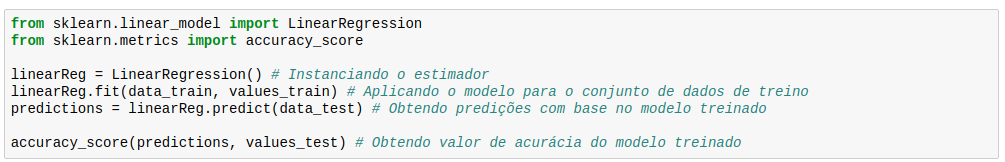
\includegraphics[scale=0.55]{figs/exemplo-scikit.png}
\label{f.exemplo-scikit}
\legend{\small Fonte: Elaborada pelo autor.}
\end{figure}


\subsection{Numpy}
\label{ss.numpy}

O NumPy é uma biblioteca, integrante do conjunto Scipy, feita em cima da biblioteca Numeric. Seu objetivo é fornecer várias funções e estruturas de dados que possam facilitar o uso da linguagem Python em um contexto científico. Teve sua primeira versão lançada em 2005, e atualmente se encontra na versão 1.15.1. \cite{numpy}

Algumas de suas funcionalidades são:

\begin{itemize}
  \item  Um poderoso objeto vetor de N-dimensões (denominado Numpy Array);
  \item Métodos para se trabalhar com vetores de maneiras mais sofisticadas;
  \item Funções de álgebra linear, transformações de Fourier e ferramentas para trabalhar com numeros aleatorios;
  \item Ferramentas de integração para códigos em Fortran e C/C++;
\end{itemize}

O NumPy se destaca por ser a base de várias outras bibliotecas científicas do Python, como o próprio Scikit que utiliza as estruturas de Numpy Array para seus cálculos.  

\subsection{Pandas}
\label{ss.pandas}

O Pandas é uma biblioteca que busca suprir uma demanda que a linguagem Python não tem por padrão, através de uma poderosa e robusta estrutura para se trabalhar com uma grande quantidade de dados estruturados, muito utilizados nas áreas de Estatística, Mercado Financeiro, Data Science, entre outros. \cite{pandas-article} O Pandas se destaca por ser baseado no NumPy, sendo assim muito facilmente integrado com todas as outras bibliotecas de ML em Python, e também por ser muito rápido e eficiente.

O Pandas apresenta duas estruturas de dados principais, \textit{Series} e \textit{Data Frames}, sendo a primeira uni-dimensional e a segunda bi-dimensional. Dentre essas duas se destaca o \textit{Data Frame}, similar ao \textit{data.frame} que está presente nativamente para a linguagem R, porém com algumas melhorias. A figura \ref{f.exemplo-pandas} ilustra um exemplo de uso desta estrutura.

Algumas das principais funções do Pandas são:

\begin{itemize}
    \item Fácil manipulação de dados nulos;
    \item Várias opções para leitura de arquivos, como por exemplo tabelas Excel, CSV, tabelas de Bancos de Dados, além de leitura de dados estruturados em arquivos HTML
    \item Inserção e remoção de colunas;
    \item Redimensionamento e obtenção de subsets;
    \item Muitos métodos utilizados no contexto de Bancos de Dados, como merge, join e groupby.
\end{itemize}

\begin{figure}[h]
\caption{\small Exemplo de utilização do Pandas.}
\centering
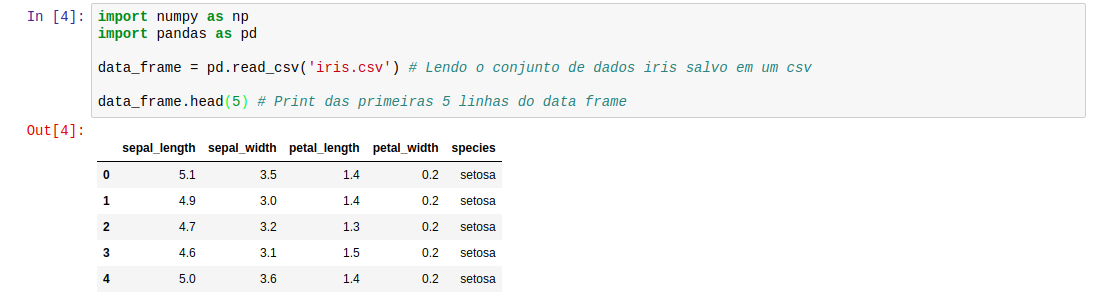
\includegraphics[scale=0.40]{figs/exemplo-pandas.png}
\label{f.exemplo-pandas}
\legend{\small Fonte: Elaborada pelo autor.}
\end{figure}

\subsection{Matplotlib}
\label{ss.matplotlib}

Matplotlib é uma biblioteca para criação de visualizações 2D em Python, que começou a ser desenvolvida em 2003 por John D. Hunter. O intuito da biblioteca era atender alguns requisitos, entre eles ser possível de ser integrado a uma interface gráfica, funcionar em diversas plataformas, oferecer suportes para publicações e funcionar em aplicações interativas. \cite{matplotlib}

O Matplotlib funciona com uma inteface similar ao do MATLAB, através do módulo pyplot. Com ele, é possível em poucas linhas ser capaz de gerar histogramas, gráficos de barra, gráficos de dispersão, entre outros.  A figura \ref{f.exemplo-matplotlib} demonstra a geração de m gráfico utilizando a biblioteca.

Além disso, os gráficos são altamente customizáveis, oferecendo controle total de elementos como estilos de linha, propriedades dos eixos, etc.

\begin{figure}[h]
\caption{\small Exemplo de utilização do Matplotlib.}
\centering
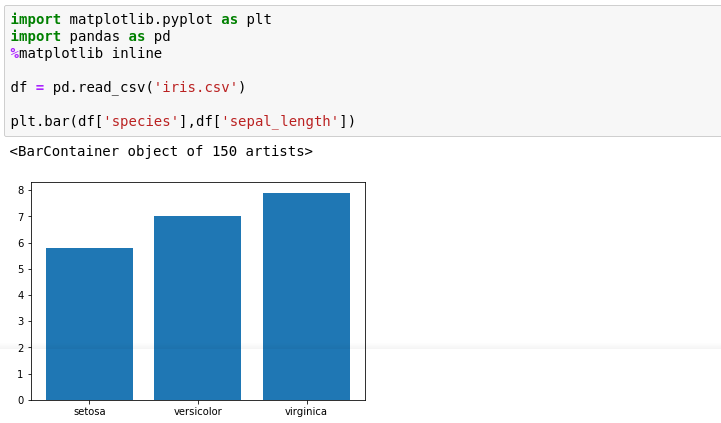
\includegraphics[scale=2]{figs/exemplo-pyplot.png}
\label{f.exemplo-matplotlib}
\legend{\small Fonte: Elaborada pelo autor.}
\end{figure}

\subsection{Seaborn}
\label{ss.seaborn}

O Seaborn é uma biblioteca Python, que funciona como um \textit{wrapper} para o Matplotlib. Ele busca simplificar ainda mais a geração de gráficos, oferecendo uma interface ainda mais simplificada que permite com que visualizações sejam geradas com apenas uma linha de código, como demonstrado na figura \ref{f.exemplo-seaborn}. Ele incorpora alguns tipos de gráficos mais avançados como Gráficos de Calor e Gráficos de violino, e também por padrão customiza os gráficos de uma maneira mais elegante, mesmo que eles tenham sido gerados usando somente o Matplotlib.

Todas as customizações são feitas através de parâmetros de função, e além disso é possível utilizar chamadas da biblioteca do Matplotlib para maiores customizações.

Além disso, o Seaborn traz em sua biblioteca um conjunto de \textit{datasets}, o que facilita na hora de se estudar as possibilidades de visualizações e entender relações entre variáveis.

\begin{figure}[h]
\caption{\small Exemplo de utilização do Seaborn.}
\centering
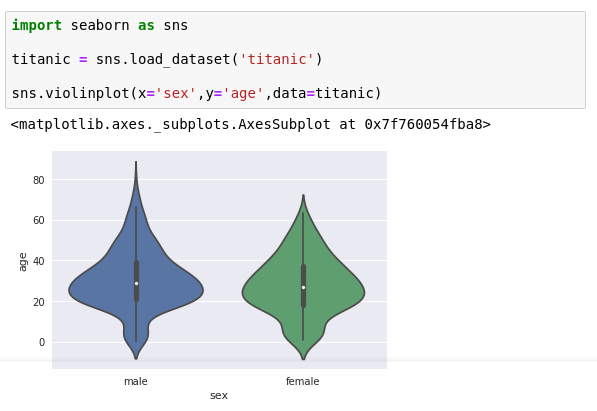
\includegraphics[scale=2.5]{figs/exemplo-seaborn.png}
\label{f.exemplo-seaborn}
\legend{\small Fonte: Elaborada pelo autor.}
\end{figure}

\subsection{Jupyter Notebook}
\label{ss.jupyter}

O Jupyter Notebook é uma aplicação \textit{web open-source}, que permite a criação de documentos, denominados Notebooks, que contenham códigos, equações, visualizações e textos explicativos. Iniciado em 2014, foi construído com base no projeto IPython, porém hoje já apresenta suporte para mais de 50 linguagens que variam de C++ até Bash. 

Um Notebook pode ser pensado como uma evolução dos consoles do tipo REPL (Read Evaluate Print Loop), que permitem com que comandos fossem inseridos de maneira interativa e seus respectivos outputs pudessem ser visualizados em tempo real, como observado pelo uso da ferramenta IPython na Figura \ref{f.exemplo-ipython}. O grande diferencial é que os arquivos do Jupyter permitem que as saídas de códigos sejam mais do que simples textos, apresentando suporte para imagens, controles e gráficos interativos e equações matemáticas formatadas. \cite{Kluyver:2016aa} 

\begin{figure}[h]
\caption{\small Exemplo de utilização do IPython.}
\centering
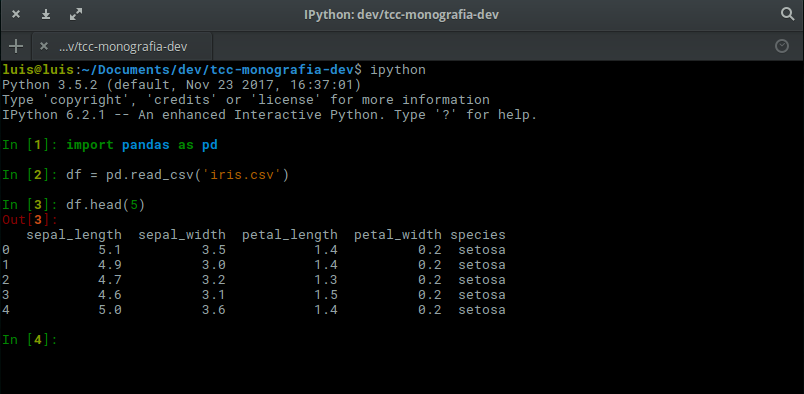
\includegraphics[scale=0.40]{figs/exemplo-ipython.png}
\label{f.exemplo-ipython}
\legend{\small Fonte: Elaborada pelo autor.}
\end{figure}

Os Notebooks foram pensados com o ambiente científico em mente, permitindo com que seja muito fácil visualizar e analisar dados facilitando o processo de desenvolvimento, assim como o posterior compartilhamento e publicação de modelos, tendo em vista que uma pessoa é capaz de não só visualizar todo o processo de criação do modelo assim como seus outputs e quaisquer textos de explicação adicionados pelo autor, mas também ser capaz de reproduzí-los em seu próprio ambiente simplesmente executando os códigos novamente.

Além disso, existem várias ferramentas que fazem com que o compartilhamento e acesso de Notebooks seja facilitado. Exemplos são o nbconvert, que converte o arquivo para os formatos HTML, PDF e LaTex, e o nbviewer que permite que \textit{Notebooks} hospedados na internet sejam visualizados no navegador sem necessidade de \textit{download}.

A execução do Jupyter se dá pela linha de comando, no diretório onde os arquivos estão presentes. Depois de executado, uma interface será aberta no navegador permitindo com que os arquivos sejam abertos e editados.

% \begin{figure}[h]
% \caption{\small Exemplo de execução do Jupyter no ambiente local.}
% \centering
% 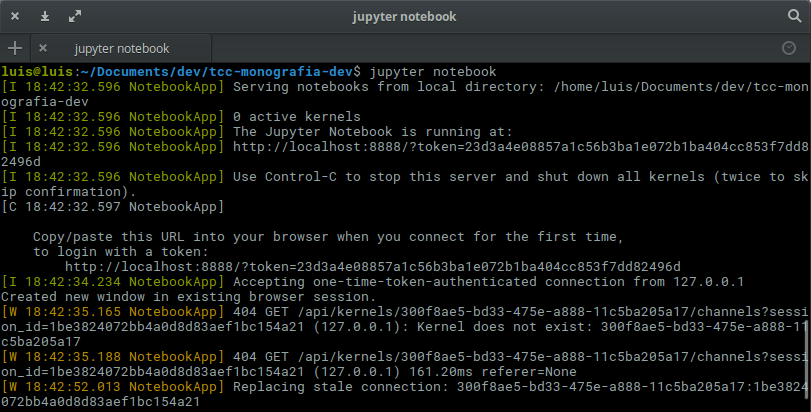
\includegraphics[scale=0.40]{figs/exemplo-jupyterutil.png}
% \label{f.exemplo-jupyterlocal}
% \legend{\small Fonte: Elaborada pelo autor.}
% \end{figure}

% \begin{figure}[h]
% \caption{\small Demonstração de interface do Jupyter.}
% \centering
% 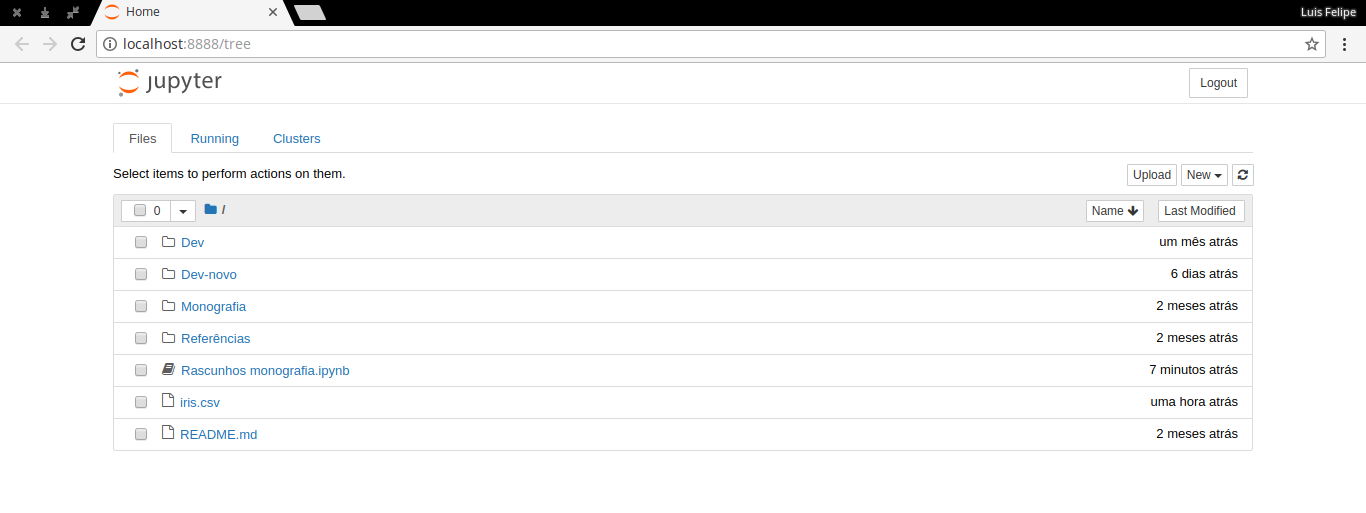
\includegraphics[scale=0.25]{figs/exemplo-jupyterinterface1.png}
% \label{f.exemplo-jupyterinterface}
% \legend{\small Fonte: Elaborada pelo autor.}
% \end{figure}
